\documentclass{article}
\usepackage{amsmath}
\usepackage{amssymb}
\usepackage[a4paper, top=25mm, bottom=25mm, left=25mm, right=25mm]{geometry}
\usepackage{pgfplots}
\usepackage{mathtools}
\usepgfplotslibrary{fillbetween}
\pgfplotsset{compat=1.18}

\begin{document}
\pagestyle{empty}
\large

\begin{center}
2020-2021 Fall\\MAT123 Midterm\\(30/11/2020)
\end{center}

\noindent 1. Evaluate $\displaystyle\lim_{x\to0^+}(\sqrt x)^{\ln(x+1)}$.

\hfill

\noindent 2. Show that the function $f(x)$ defined by

\[
f(x)=
\begin{cases}
\displaystyle x\arctan\frac{1}{x},&\text{if}\ x>0\\[1em]
0,&\text{if}\ x=0\\[1em]
\displaystyle \frac{x-\cos x}{x^2},&\text{if}\ x<0
\end{cases}
\]

\noindent is not continuous at the point $x=0$.

\hfill

\noindent 3. Find an equation of the line which is tangent to the curve

\[\cos y^2+xy+1=0\]

\noindent at the point $\left(\sqrt{\dfrac{2}{\pi}},-\sqrt{\dfrac{\pi}{2}} \right)$. Note that $y=f(x)$.

\hfill

\noindent 4. A block of ice in the shape of a cube originally having volume of $3000$ cm$^3$. When it is melting, the surface area is decreasing at the rate of 36 cm$^2$/h. At what rate does the length of each of its edges decrease at the time its volume is 216 cm$^3$? Assume that during melting, the block of ice maintains its cubical shape.

\hfill

\noindent 5.

\hfill

\noindent (a) Using the Intermediate Value Theorem and Rolle’s theorem, show that the equation $e^x + x = 0$ has only one root (Note that if this root $c_1$, then $c_1\in(-1,0)$).

\hfill

\noindent (b) Determine the interval of increase, decrease, and concavity of the function $f(x)=\mathrm e^x+x$. By constructing a table, sketch the graph.

\hfill

\noindent 6. Determine (but do not evaluate) the integral corresponding to the area of the region bounded by the curves $y=-x^2+1$ and $y =|x|-1$.

\hfill

\noindent 7. Evaluate $\displaystyle\int x\ln x\,dx$.

\hfill

\newpage

\begin{center}
2020-2021 Fall Midterm (30/11/2020) Solutions\\
(Last update: 29/08/2025 22:18)
\end{center}

\noindent 1. Let $L$ be the value of the limit. Since the expression is continuous for $x>0$, we can apply the logarithm function to each side of the equation. Then, we can swap the logarithm and the limit. Use the property of logarithms afterwards.

\[L=\lim_{x\to0^+}\left(\sqrt x\right)^{\ln\left(x+1\right)}\]

\[\ln(L)=\ln\left[\lim_{x\to0^+}\left(\sqrt x\right)^{\ln\left(x+1\right)}\right]=\lim_{x\to0^+}\ln\left[\left(\sqrt x\right)^{\ln\left(x+1\right)}\right]=\lim_{x\to0^+}\ln\left[\left(\sqrt x\right)^{\ln\left(x+1\right)}\right] \]
\[\ln\left(L\right)=\lim_{x\to0^+}\left[\ln\left(x+1\right)\cdot\ln\left(\sqrt x\right)\right] \quad\left[0\cdot\infty\right]\]

\hfill

\noindent Make it so the limit is in the form $\displaystyle \frac00$ or $\displaystyle \frac\infty\infty$ in order to apply the L'Hôpital's rule.

\begin{align*}\ln\left(L\right)&=\lim_{x\to0^+}\left[\frac{\ln\left(\sqrt x\right)}{\frac1{\ln\left(x+1\right)}}\right] \quad\left[\frac\infty\infty\right]\\\\&\overset{\text{L'H.}}{=}\lim_{x\to0^+}\left[\frac{\frac1{\sqrt x}\cdot\frac1{2\sqrt x}}{-\frac1{\ln^2\left(x+1\right)}\cdot \frac1{x+1}}\right]=\lim_{x\to0^+}\left[-\frac{\ln^2(x+1)\cdot(x+1)}{2x}\right]\\\\&=\lim_{x\to0^+}\left[-\frac{\ln^2(x+1)}{2x}\right] \cdot\lim_{x\to0^+} \left(x+1\right)=\lim_{x\to0^+}\left[-\frac{\ln^2(x+1)}{2x}\right]\quad\left[\frac00\right]\\\\&\overset{\text{L'H.}}{=}\lim_{x\to0^+}\left[-\frac{2\ln(x+1) \cdot\frac1{x+1}}2\right]=\lim_{x\to0^+}\left[\frac{\ln(x+1)}{x+1}\right]=\frac{\ln1}{1}=0\end{align*}

\hfill

\noindent $\ln(L)=0$, so $\boxed{L=1}$.

\hfill

\noindent 2. $\displaystyle \arctan\frac1x$ takes it values on $\displaystyle -\frac{\pi}2 \leq \arctan\frac1x \leq \frac{\pi}2$. Multiply each side by $x$, then we get $\displaystyle -\frac{x\pi}2 \leq x\arctan\frac1x \leq \frac{x\pi}2$. Take the limits of each side. By the squeeze theorem, we see that the limit of $\displaystyle x\arctan\frac1x$ at the point $x=0$ is $0$. This means that for $f(x)$, the limit from the right side also equals $0$.

\[\lim_{x\to 0}\left(-\frac{x\pi}2\right)\leq\lim_{x\to 0}\left(x\arctan\frac1x\right)\leq\lim_{x\to 0}\left(\frac{x\pi}2\right)\]
\[0\leq\lim_{x\to 0}\left(x\arctan\frac1x\right)\leq0\]
\[\therefore\lim_{x\to 0}\left(x\arctan\frac1x\right) = 0\]

\hfill

\noindent From the left side, the limit is equal to as follows.

\[\lim_{x\to0^-}\frac{x-\cos x}{x^2}=\lim_{x\to0^-}(x-\cos x)\cdot\lim_{x\to0^-}\frac1{x^2} =-\infty\]

\hfill

\noindent Continuity requires the equality of one-sided limits and the value of the function at that point. However, the one-sided limits are not equal; $0\neq-\infty$. Therefore, $f(x)$ is discontinuous at $x=0$.

\hfill

\noindent 3. Differentiate both sides implicitly.

\[\frac{d}{dx}\left(\cos y^2+xy+1\right)=\frac{d}{dx}(0)\]
\[-\sin y^2\cdot2y\frac{dy}{dx}+y+x\frac{dy}{dx}=0\]

\[\frac{dy}{dx}\left(-\sin y^2\cdot2y+x\right)=-y\]

\begin{equation}\frac{dy}{dx}= \frac y{\sin y^2 \cdot 2y - x}\end{equation}

\hfill

\noindent Evaluate $\displaystyle \frac{dy}{dx}$ at the point.

\begin{equation}\left.\frac{dy}{dx}\right|_{\left(\sqrt{\frac{2}{\pi}},-\sqrt{\frac{\pi}{2}}\right)} =\frac y{\sin y^2\cdot2y-x}=\frac{-\sqrt{\frac{\pi}{2}}}{\sin\left(\left(-\sqrt{\frac{\pi}{2}}\right)^2\right)\cdot2\left(-\sqrt{\frac{\pi}{2}}\right)-\sqrt{\frac{2}{\pi}}} =\frac{\sqrt{\frac{\pi}{2}}}{\sqrt{2\pi}+\sqrt{\frac{2}{\pi}}}\end{equation}

\hfill

\noindent Recall: $y-y_0 = m(x-x_0)$, where $m$ is the slope. Substitute $m$ with $(2)$ and find the tangent line.

\[\boxed{y+\sqrt{\frac{\pi}{2}}=\frac{\displaystyle\sqrt{\frac{\pi}{2}}}{\displaystyle\sqrt{2\pi}+\sqrt{\frac{2}{\pi}}}\left(x-\sqrt{\frac{2}{\pi}}\right)}\]

\hfill

\noindent 4. Let $S(t),\, V(t),\, a(t)$ represent the surface area, the volume, and the length of one side of the object, respectively, as a function of time. We may write the following.

\[S(t)=6a^2(t),\quad V(t)=a^3(t)\]

\hfill

\noindent Given that at $t=t_0$, $V(t_0) = 216, \,S'(t_0)=-36$. Using the relationship with the sides,

\begin{align*}
&V(t_0) = a^3(t_0)= 216\,\rightarrow\, a(t_0) = 6\\
&S'(t_0) = 12a(t_0)a'(t_0)=-36\\
&\therefore 12\cdot6\cdot a'(t_0)=-36 \,\rightarrow\, a'(t_0)=-\frac12
\end{align*}

\[\boxed{a'(t_0) = -\frac12\,\text{cm/h}}\]

\newpage

\noindent 5.

\hfill

\noindent (a) Let $f(x) = \mathrm{e}^x + x$. $f$ is continuous and differentiable for all $x\in\mathbb{R}$.

\[f(-1)=\mathrm{e}^{-1}-1=\frac1{\mathrm{e}}-1,\quad f(0)=\mathrm{e}-0=\mathrm{e}\]

\hfill

\noindent Since $f(-1) < 0$ and $f(0) > 0$ and $f$ is continuous on the interval $[-1, 0]$, by IVT, there is at least one point $x_1$ that satisfies $f(x_1) = 0$. Assume that there is another distinct root $x_2$. Rolle's theorem states that if $f$ is continuous on a particular interval with endpoints having the same function value, there exists a point $c$ on that interval such that $f'(c) = 0$ there.

\[f'(c)=\mathrm{e}^c+1\geq1\qquad\left[\mathrm{e}^c>0\right]\]

\hfill

\noindent This yields a contradiction. Therefore, there is \textit{only} one root.

\hfill

\noindent (b) The expression is defined $\forall x\in\mathbb{R}$. Let us find the limit at infinity and the limit at negative infinity.

\[\lim_{x\to\infty}\left(\mathrm{e}^x+x\right)=\infty\qquad\lim_{x\to-\infty}\left(\mathrm{e}^x+x\right)=-\infty\]

\hfill

\noindent There are no vertical or horizontal asymptotes. However, there is a slant asymptote. Attempt a long polynomial division and we will find that the slant asymptote is $y=x$. Verify with the following limit:

\[\lim_{x\to-\infty}\left[\left(\mathrm{e}^x+x\right)-x\right]=\lim_{x\to-\infty}\mathrm{e}^x=0\]

\hfill 

\noindent Take the first and second derivatives.

\[y'=\mathrm{e}^x+1,\quad y''=\mathrm{e}^x\]

\hfill 

\noindent We see that there are no critical or inflection points either. Now, set up a table and see what the graph looks like.

\begin{center}
    \large
    \begin{tabular}{ |c| c| } 
    \hline
        $x$ & $(-\infty, \infty)$\\
        \hline
        $y$ & $(-\infty, \infty)$\\
        \hline
        $y'$ sign & + \\
        \hline
        $y''$ sign & + \\
        \hline
    \end{tabular}
\end{center}

\hfill

\begin{center}
\begin{tikzpicture}
  \begin{axis}[
    axis lines = center,
    xlabel = $x$, ylabel = $y$,
    domain=-4:4,
    samples=200,
    ymin=-4, ymax=4,
    xmin=-4, xmax=4,
    axis line style={->},
    scale=1.3,
    ]
    \addplot[blue, thick] {e^x+x};
    
    \node[blue] at (1.8, 3.2) {$y=\mathrm e^x+x$};

    \draw[dashed, red] (axis cs:-5,-5) -- (axis cs:5,5);
  \end{axis}
\end{tikzpicture}
\end{center}

\noindent 6.
\begin{center}
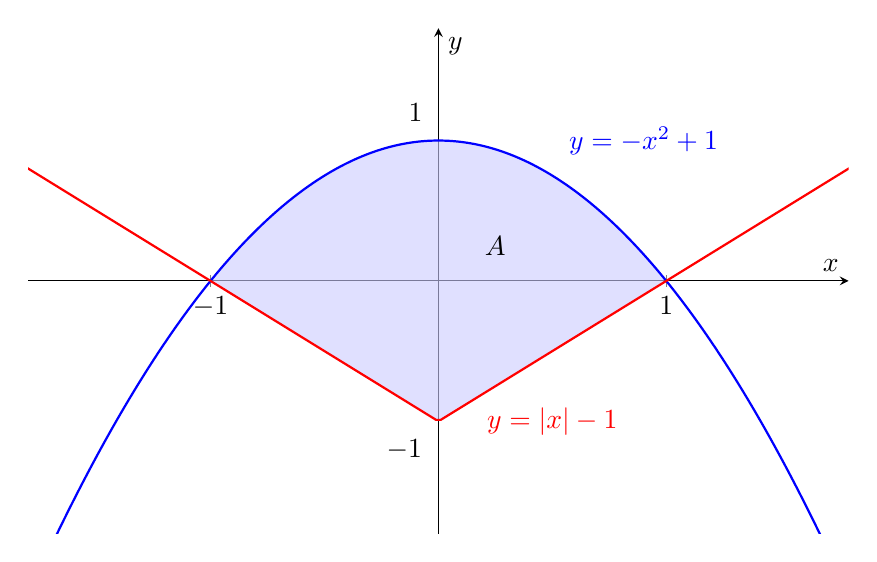
\begin{tikzpicture}
  \begin{axis}[
    axis lines = middle,
    xlabel = $x$,
    ylabel = $y$,
    domain=-2:2,
    samples=200,
    xtick={-2,-1,1,2},
    ytick={2,-2},
    ymin=-1.8, ymax=1.8,
    xmin=-1.8, xmax=1.8,
    width=12cm,
    height=8cm,
  ]

    \addplot [
      name path=upper,
      domain=-1:1,
      samples=200,
      draw=none
    ] {-x^2 + 1};

    \addplot [
      name path=lower,
      domain=-2:2,
      samples=200,
      draw=none
    ] {abs(x) - 1};

    \addplot [
      fill=blue!20,
      draw=none,
      opacity=0.6,
    ] fill between[of=upper and lower, soft clip={domain=-2:2}];

    \addplot [thick, blue] {-x^2 + 1};
    \addplot [thick, red] {abs(x) - 1};
    
    \node at (-0.1, 1.2) {$1$};
    \node at (-0.15, -1.2) {$-1$};
    
    \node[blue] at (0.9, 1) {$y=-x^2+1$};
    \node[red] at (0.5, -1) {$y=|x|-1$};
    
    \node at (0.25, 0.25) {$A$};

  \end{axis}
\end{tikzpicture}
\end{center}

\hfill

\noindent The area of the region is as follows.

\[A=\int_{-1}^1\left[(-x^2+1)-(|x|-1)\right]\,dx=\int_{-1}^0(-x^2+x +2)\,dx+\int_{0}^1(-x^2-x+2)\,dx\]

\hfill

\noindent 7. We'll use integration by parts.

\[
\left.
\begin{array}{ll}
\displaystyle\ln x=u\,\rightarrow\,\frac1x\,dx=du  \\
\displaystyle x\,dx= dv \,\rightarrow\,\frac{x^2}2=v
\end{array}
\right\}\quad
\begin{array}{ll}
\mathrm{I}&=\displaystyle\int x\ln x\,dx = \frac{x^2}2\cdot\ln x-\int\frac{x^2}2\cdot \frac1x \,dx \\\\&=\displaystyle\frac{x^2}2\cdot\ln x-\int\frac{x}2\,dx=\boxed{\frac{x^2}2\cdot\ln x - \frac{x^2}4+c,\,c\in\mathbb{R}}
\end{array}
\]

\end{document}